%!TEX root=nips_2016.tex
\section{Experiments}
We now show the power of our adversarial modeling framework for generating discrete sequences. To illustrate this we consider modeling the context-free grammar introduced in Section 3. We generate $5000$ samples with a maximum length of $12$ characters from the context-free grammar (CFG) for our training set. We pad all sequences with less than $12$ characters with spaces.

\subsection*{Optimization details}
We train both the discriminator and generator using ADAM \cite{kingma2014adam} with a fixed learning rate of $0.001$ and a mini-batch size of $m\!=\!200$. Inspired by the work of \cite{sonderby2016amortised} who use input noise to stabilize GAN training, for every input $\x$ we form a vector $\mathbf{h}$ such that its softmax (instead of being one-hot) places a probability of approximately $0.9$ on the correct character and a probability of $(1-0.9)/(d-1)$ on the remaining $d\!-\!1$ characters. We then apply the Gumbel-softmax trick to generate a vector $\mathbf{y}$ as in equation~(\ref{sec:gumbel:eq:2}). We use this vector instead of $\x$ throughout training. We train the generator and discriminator for $20,000$ mini-batch iterations. During the training we linearly anneal the temperature of the Gumbel-softmax distribution, from $\tau\!=\!5$ (i.e., a very flat distribution) to $\tau\!=\!1$ (a more peaked distribution) for iterations $1$ to $10,000$ and then kept at $\tau\!=\!1$ until training ends. 


\begin{figure*}[t!]
\begin{center}
\centerline{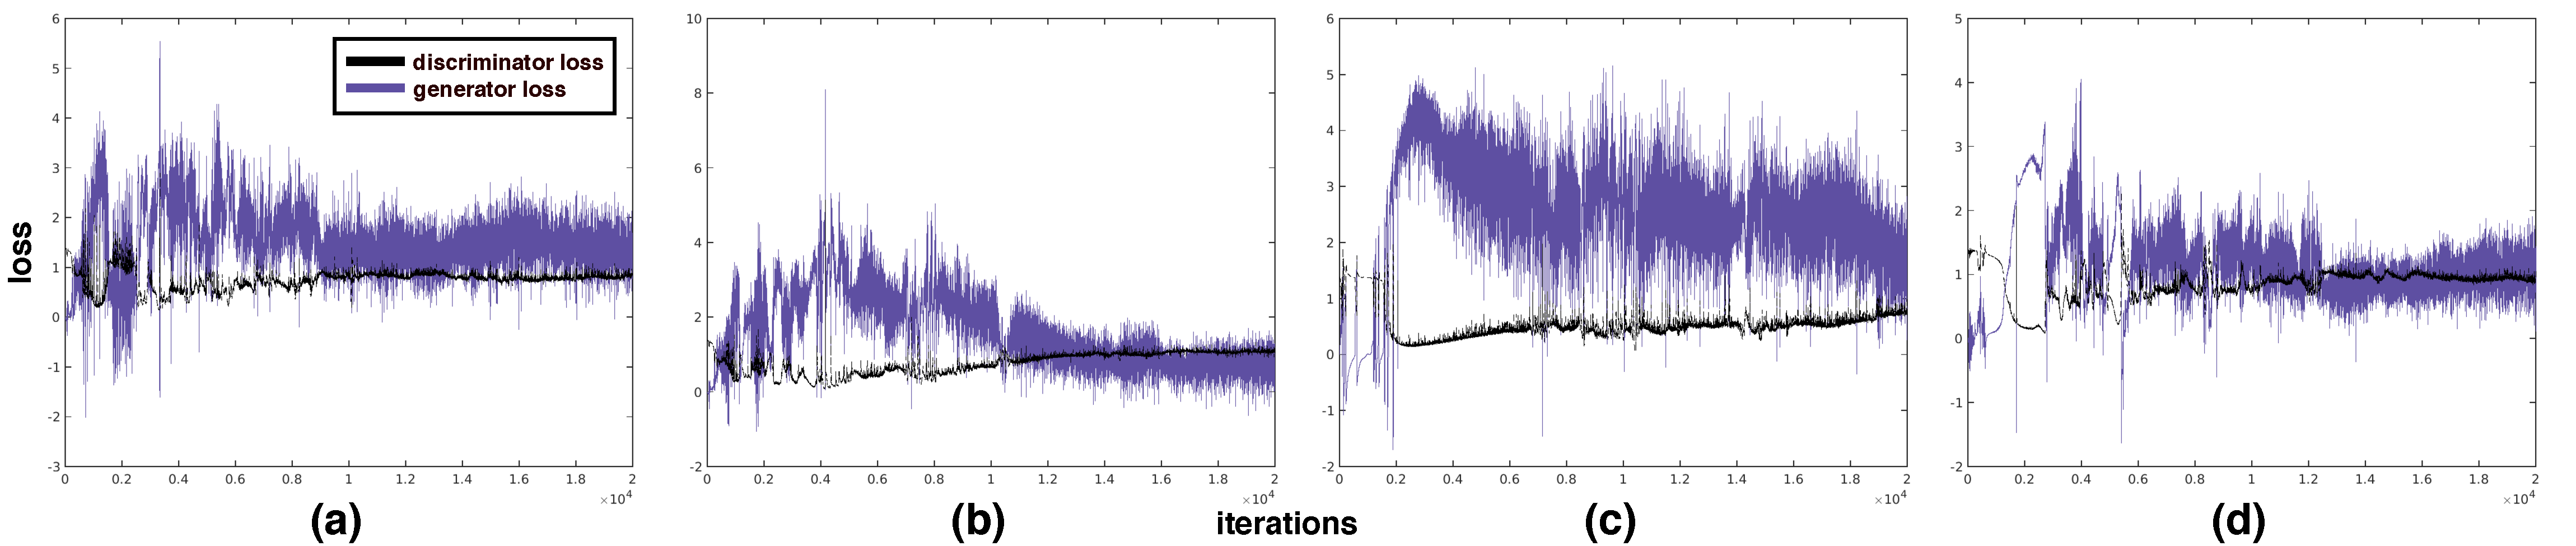
\includegraphics[width=\textwidth]{gan_losses.pdf}}
\vspace{-2ex}
\caption{The generative and discriminative losses throughout training. Ideally the loss of the discriminator should increase while the generator should decrease as the generator becomes better at mimicking the real data. \textbf{(a)} The default network with Gumbel-softmax temperature annealing. \textbf{(b)} The same setting as (a) but increasing the size of the generated samples to $1,000$. \textbf{(c)} Only varying the input vector temperature. \textbf{(d)} Only introducing random noise into the hidden state and not the cell state.}
%\vspace{-5ex}
\label{figure.losses}
\end{center}
\end{figure*}

\subsection*{Learning a CFG}
Figure~\ref{figure.losses} \textbf{(a)} shows the generator and discriminator losses throughout training for this setting. We experimented with increasing the size of the generated samples to $1,000$, as this has been reported to improve GAN modeling \cite{huszar2015not}, shown in Figure~\ref{figure.losses} \textbf{(b)}. We also experimented with just varying the temperature for the input vectors $\mathbf{y}$ and fixing the generator temperature to $\tau\!=\!1$ (in Figure~\ref{figure.losses} \textbf{(c)}).  Finally, we also tried just introducing random noise into the hidden state and allowing the network to learn an initial cell state $C_0$ (Figure~\ref{figure.losses} \textbf{(d)}).

\begin{figure*}[t!]
\begin{center}
\centerline{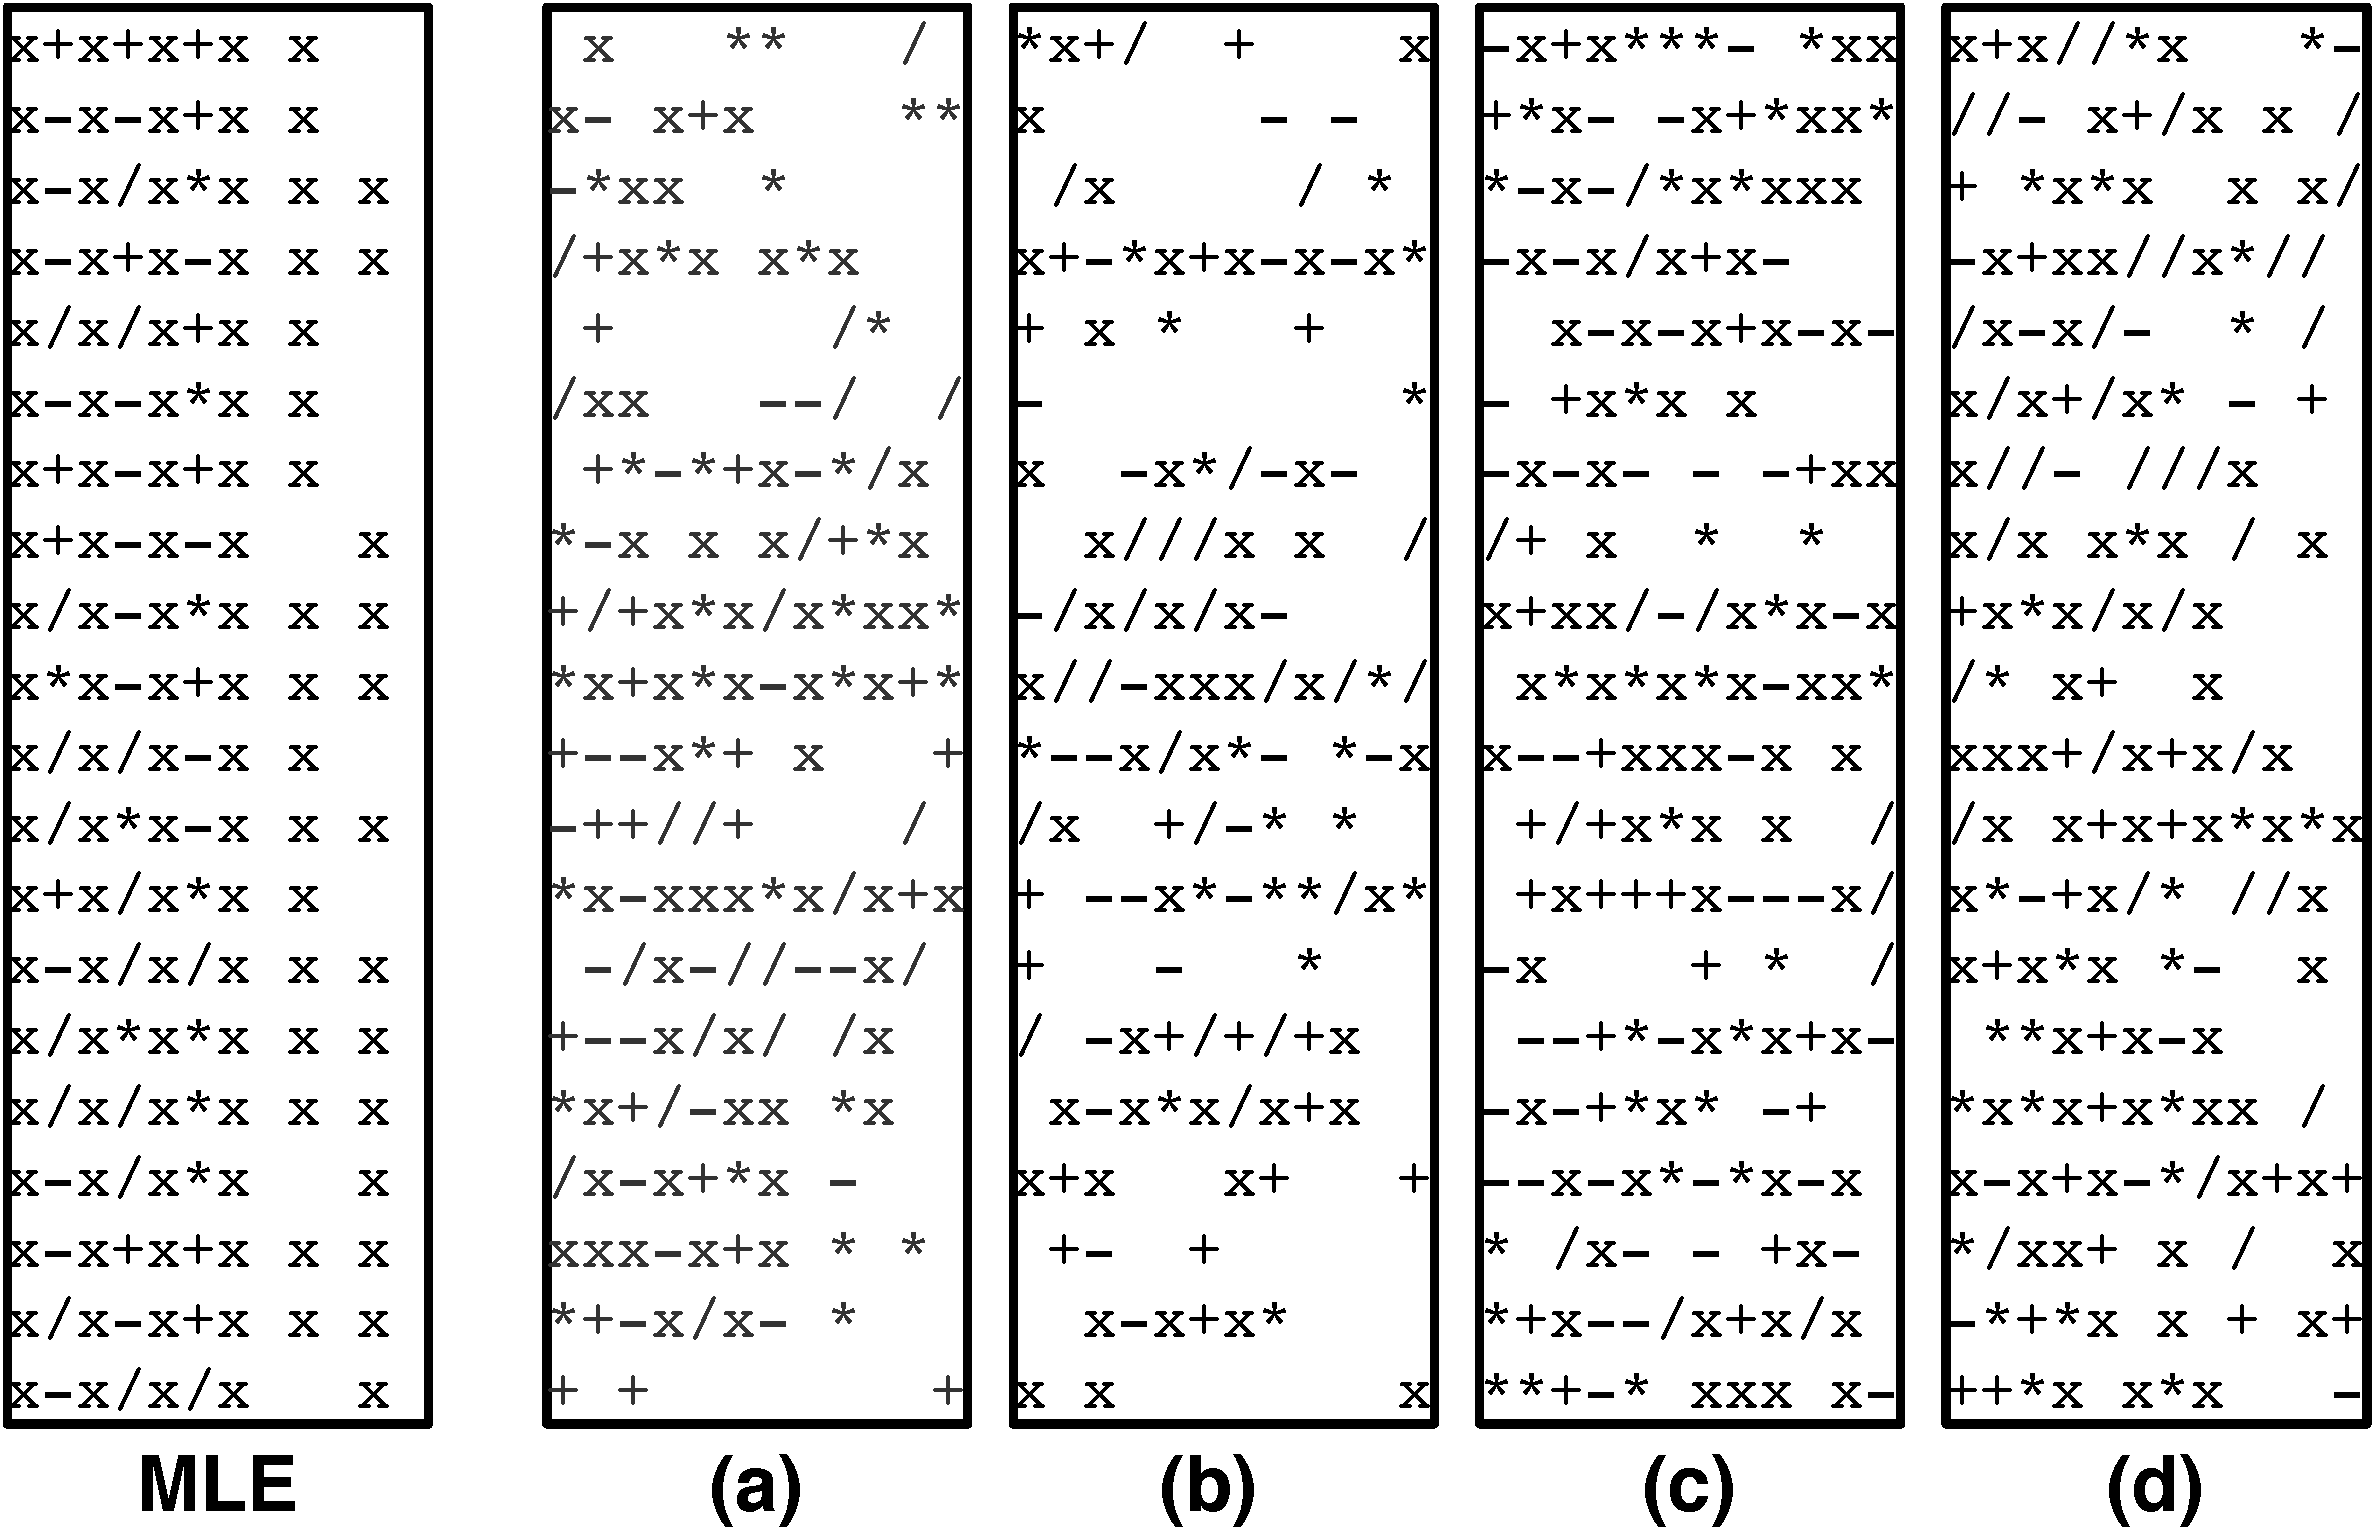
\includegraphics[width=\textwidth]{generated.pdf}}
\vspace{-2ex}
\caption{The generated text for MLE and GAN models. The plots \textbf{(a)}-\textbf{(d)} correspond to the models of Figure~\ref{figure.losses}.}
%\vspace{-5ex}
\label{figure.generate}
\end{center}
\end{figure*}

Figure~\ref{figure.generate} shows the text generated by MLE and GAN models. Each row is a sample from either model, each consisting of $12$ characters (we have included the blank space character as some training inputs are padded with spaces if less than $12$ characters). While the MLE LSTM is not strictly a generative model in the sense of drawing a discrete sequence from a distribution, we include it for reference. We can see that our GAN models are learning to generate alternating sequences of $x$'s, similar to the MLE result. Specifically, the 4th, 10th, and 17th rows of plot \textbf{(a)}, show samples that are very close to the training data, and many such examples exist for the remaining plots as well. 

We believe that these results, as a proof of concept, show strong promise for training GANs to generate discrete sequence data. Further, we believe that incorporating recent advances in GANs such as training GANs using variational divergence minimization \cite{nowozin2016f} or via density ratio estimation \cite{uehara2016generative} could yield further improvements. We aim to experiment with these in future work.
